
%(BEGIN_QUESTION)
% Copyright 2011, Tony R. Kuphaldt, released under the Creative Commons Attribution License (v 1.0)
% This means you may do almost anything with this work of mine, so long as you give me proper credit

A PLC counts packages coming by on a conveyor belt in a manufacturing facility.  An optical sensor detects these packages as they travel by on the conveyor belt:

$$\includegraphics[width=15.5cm]{i03596x01.eps}$$

Unfortunately, something is not working correctly in this system.  The HMI display continues to read a count value of zero no matter how many packages pass by the sensor switch.  This very same system worked just fine three days ago, and had been working fine for one whole year before that..

\vskip 10pt

Brainstorm at least five different faults that could account for this problem, and then devise a ``next test'' you would conduct to narrow the field of potential faults.  The simpler this test (i.e. the least amount of time to conduct and the less complicated test equipment required), the better!

\vskip 10pt

\begin{itemize}
\item{} 
\vskip 20pt
\item{} 
\vskip 20pt
\item{} 
\vskip 20pt
\item{} 
\vskip 20pt
\item{} 
\end{itemize}

\vskip 10pt

\noindent
{\bf Next test}:

\vfil 

\vskip 20pt \vbox{\hrule \hbox{\strut \vrule{} {\bf Suggestions for Socratic discussion} \vrule} \hrule}

\begin{itemize}
\item{} Explain how your proposed diagnostic test would either confirm or eliminate certain fault possibilities.
\end{itemize}

\underbar{file i03596}
\eject
%(END_QUESTION)





%(BEGIN_ANSWER)


%(END_ANSWER)





%(BEGIN_NOTES)

Here is a list of faults, by no means exhaustive:

\begin{itemize}
\item{} Light source burned out
\item{} Dirty lens on sensor switch
\item{} Broken wire between sensor and PLC input
\item{} Failed PLC input channel
\item{} Halted PLC program
\item{} Failed communication cable between PLC and HMI
\item{} Failed HMI display (frozen)
\end{itemize}

A great ``next test'' would be to check the input LED indicator on the PLC input, to see whether or not the PLC is receiving a pulse signal from the sensor for every passing package.

%INDEX% PLC, troubleshooting: conveyor package-counting system with HMI

%(END_NOTES)


